\chapter{Конструкторский раздел}

\section{Модель оценки трудоемкости алгоритмов}
Введем модель оценки трудоемкости.

\begin{enumerate}
	\item Трудоемкость базовых операций.
	
	Пусть трудоемкость следующих операций равной 2: 
	$$
		\label{eq3:1}
		*, /, \, //, \%, *=, /=
	$$
	
	Примем трудоемкость следующих операций равной 1:
	
	$$
		\label{eq3:2}
		=, +, -, +=, -=, ==, !=, <, >, \leq, \geq, |, \&\&,, ||, [\ ]
	$$

	\item Трудоемкость цикла.
	
	Пусть трудоемкость цикла определяется по формуле (\ref{eq3:3}).
	
	\begin{equation}
		\label{eq3:3} 
		f = f_{init} + f_{comp} + N_{iter} * (f_{in} + f_{inc} + f_{comp})
	\end{equation} 
	где:
	\begin{itemize}
		\item $f_{init}$ - трудоемкость инициализации переменной-счетчика;
		\item $f_{comp}$ - трудоемкость сравнения;
		\item $N_{iter}$ - номер выполняемой итерации;
		\item $f_{in}$ - трудоемкость команд из тела цикла;
		\item $f_{inc}$ -трудоемкость инкремента;
		\item $f_{comp}$ - трудоемкость сравнения.
	\end{itemize}
	\item Трудоемкость условного оператора. \\
	Пусть трудоемкость самого условного перехода равна 0, но она определяется по формуле (\ref{eq3:4}). 
	\begin{equation}
		\label{eq3:4}
		f_{if} = f_{comp\_if} +
		\begin{sqcases}
			f_{a}\\
			f_{b}\\
		\end{sqcases}
	\end{equation}
	
\end{enumerate}


\section{Вычисление трудоемкости алгоритмов}
Пусть во всех дальнейших вычислениях размер матрицы А имеет $M \times N$, для матрицы B - $N \times Q$.

\subsection{Трудоемкость алгоритма умножения матриц по Винограду}
Трудоемкость этого алгоритма вычисляется по формуле (\ref{eq3:5}).
\begin{multline}
	\label{eq3:5}
	f_{станд} = {\underset{=}{1}} + {\underset{<}{1}} + M({\underset{++}{2}} + {\underset{=}{1}} + {\underset{<}{1}} + Q({\underset{++}{2}} + {\underset{=}{1}} + {\underset{<}{1}} + N({\underset{++}{2}} + {\underset{[\ ]}{8}} + {\underset{*}{2}} + {\underset{=}{1}} + {\underset{+}{1}}))) = \\
	= 14MNQ + 4MQ + 4M + 2
\end{multline}

\subsection{Трудоемкость алгоритма умножения матриц по Винограду}
Трудоемкость этого алгоритма состоит из следующих компонентов, определяемых по формуле (\ref{eq3:6}).
\begin{equation}
	\label{eq3:6}
	f_{vin} = f_{init} + f_{precomp} + f_{fill} + f_{even}
\end{equation}
\newpage

где:
\begin{itemize}
	\item $f_{init}$ - трудоемкость инициализации массивов для предварительного вычисления (\ref{eq3:7});
	\begin{multline}
		\label{eq3:7}
		f_{init} = {\underset{=}{1}} + {\underset{<}{1}} + M({\underset{++}{2}} + {\underset{[\ ]}{1}} + {\underset{=}{1}}) + {\underset{=}{1}} + {\underset{<}{1}} + Q({\underset{++}{2}} + {\underset{[\ ]}{1}} + {\underset{=}{1}}) = \\
		= 2 + 4M + 2 + 4Q = 4 + 4M + 4Q 
	\end{multline}


	\item $f_{precomp}$ - трудоемкость предварительного заполнения строк матрицы А и столбцов матрицы B (\ref{eq3:8});
	\begin{multline}
		\label{eq3:8}
		f_{precomp} = f_{rows} + f_{columns} = {\underset{=}{1}} + {\underset{<}{1}} + M({\underset{++}{2}} + {\underset{=}{1}} + {\underset{<}{1}} + \frac{n}{2}({\underset{++}{2}} + {\underset{[\ ]}{6}} + {\underset{=}{1}} + {\underset{+}{2}} + {\underset{*}{6}})) + \\
		+ {\underset{=}{1}} + {\underset{<}{1}} + Q({\underset{++}{2}} + {\underset{=}{1}} + {\underset{<}{1}} + \frac{N}{2}({\underset{++}{2}} + {\underset{[\ ]}{6}} + {\underset{=}{1}} + {\underset{+}{2}} + {\underset{*}{6}})) = \\
		= 2 + M(4 + \frac{N}{2} * 17) + 2 + Q(4 + \frac{N}{2} * 17) = \\
		= 4 + 4M + 4Q + \frac{17NM}{2} + \frac{17NQ}{2}
	\end{multline}


	\item $f_{even}$ - трудоемкость заполнения результирующей матрицы (\ref{eq3:9});
	\begin{multline}
		\label{eq3:9}
		f_{fill} = {\underset{=}{1}} + {\underset{<}{1}} + M({\underset{++}{2}} + {\underset{=}{1}} + {\underset{<}{1}} + Q({\underset{++}{2}} + {\underset{[\ ]}{4}} + {\underset{=}{1}} + {\underset{-}{2}} + {\underset{=}{1}} + {\underset{<}{1}} +\\
		+ \frac{N}{2}({\underset{++}{2}} + {\underset{[\ ]}{12}} + {\underset{=}{1}} +
		{\underset{+}{5}} + {\underset{*}{10}} + {\underset{/}{2}})) = 2 + M(4 + Q(11 + 16N)) = \\
		= 2 + 4M + 11MQ + 16MNQ
	\end{multline}

	\item $f_{fill}$ - трудоемкость для дополнения умножения в случае нечетной размерности матрицы. (\ref{eq3:10}).
	\begin{multline}
		\label{eq3:10}
		f_{fill} = {\underset{\%}{2}} + {\underset{==}{1}} + 
		\begin{sqcases}
			{\underset{=}{1}} + {\underset{<}{1}} + M({\underset{++}{2}} + {\underset{=}{1}} + {\underset{<}{1}} + Q({\underset{++}{2}} + {\underset{[\ ]}{8}} + \\
			+ {\underset{=}{1}} + {\underset{+}{1}} + {\underset{-}{2}})),\\
			0\\
		\end{sqcases} = \\
		 = 3 + \begin{sqcases}
			2 + 4M + 14MQ,\\
			0\\
		\end{sqcases}
	\end{multline}
	
	Результирующая трудоемкость алгоритма Винограда составляет $f_{vin} \approx 16MNQ$
\end{itemize}
\subsection{Трудоемкость оптимизированного алгоритма умножения матриц по Винограду}
Трудоемкость этого алгоритма определяется из следующих компонентов по формуле (\ref{eq3:11}).
\begin{equation}
	f_{optim} = f_{init} + f_{precomp} + f_{fill}
	\label{eq3:11}
\end{equation}
где:
\begin{itemize}
	\item $f_{init}$ - определяется по формуле (\ref{eq3:7}) в добавок с другими компонентами (\ref{eq3:12});
	\begin{equation}
		f_{init} = 4 + 4M + 4Q + {\underset{=}{2}} + {\underset{\%}{2}} + {\underset{-}{1}} + {\underset{==}{1}} + 
		\begin{sqcases}
			{\underset{-=}{1}},\\
			0
		\end{sqcases} = 7 + 4M + 4Q + \begin{sqcases}
										{\underset{-=}{1}},\\
										0
									  \end{sqcases}
		\label{eq3:12}
	\end{equation}

	\item $f_{precomp}$ - трудоемкость предварительного заполнения строк матрицы А и столбцов матрицы B (\ref{eq3:13});
	\begin{multline}
		f_{precomp} = {\underset{=}{1}} + {\underset{<}{1}} + M({\underset{++}{2}} + {\underset{=}{2}} + {\underset{<}{1}} + N({\underset{+=}{2}} + {\underset{*}{2}} + {\underset{+}{1}} + {\underset{[\ ]}{4}}) + {\underset{[\ ]}{1}} + {\underset{=}{1}}) + \\
		+ {\underset{=}{1}} + {\underset{<}{1}} + Q({\underset{++}{2}} + {\underset{=}{2}} + {\underset{<}{1}} + N({\underset{+=}{2}} + {\underset{[\ ]}{4}} + {\underset{*}{2}} + {\underset{+}{1}}) + {\underset{=}{1}}) = \\
		= 2 + 7M + 9MN + 2 + 6Q + 9NQ = 9MN + 9NQ + 7M + 6Q + 4
		\label{eq3:13}
	\end{multline}

	\item $f_{fill}$ - трудоемкость для заполнения матрицы (\ref{eq3:14}).
	\begin{multline}
		f_{fill} = {\underset{=}{1}} + {\underset{<}{1}} + M({\underset{++}{2}} + {\underset{=}{2}} + {\underset{<}{1}} + Q({\underset{++}{2}} + {\underset{=}{2}} + {\underset{-}{1}} + {\underset{+}{1}} + {\underset{[\ ]}{2}} + {\underset{<}{1}} + \\
		+ \frac{N}{2}({\underset{+=}{2}} + {\underset{[\ ]}{8}} + {\underset{+}{4}} + {\underset{*}{2}}) + {\underset{==}{1}} 
		 +  \begin{sqcases}
				{\underset{+=}{1}} + {\underset{[ \ ]}{4}} + {\underset{*}{2}}\\
				0
			\end{sqcases} + {\underset{[\ ]}{2}} + {\underset{=}{1}})) = \\
		= 2 + M(4 + Q(\frac{16}{2}) + 13 + \begin{sqcases}
											6\\
											0
											\end{sqcases})) = \\
		8MNQ + 14MQ + 4M + 2 + \begin{sqcases}
									6\\
									0
									\end{sqcases} MQ
		\label{eq3:14}
	\end{multline}
	Результирующая трудоемкость оптимизированного алгоритма Винограда для лучшего и худшего случая составляет (\ref{eq3:15}).
	\begin{equation}
		f_{fill} \approx 8MNQ
		\label{eq3:15}
	\end{equation}
	
\end{itemize}

\section{Схемы алгоритмов умножения матриц}
Ниже представлены следующие схемы алгоритмов:
\begin{itemize}
	\item рис. \ref{png:1} - схема алгоритма стандартного умножения матриц;
	\begin{figure}[H]
		\centering{
			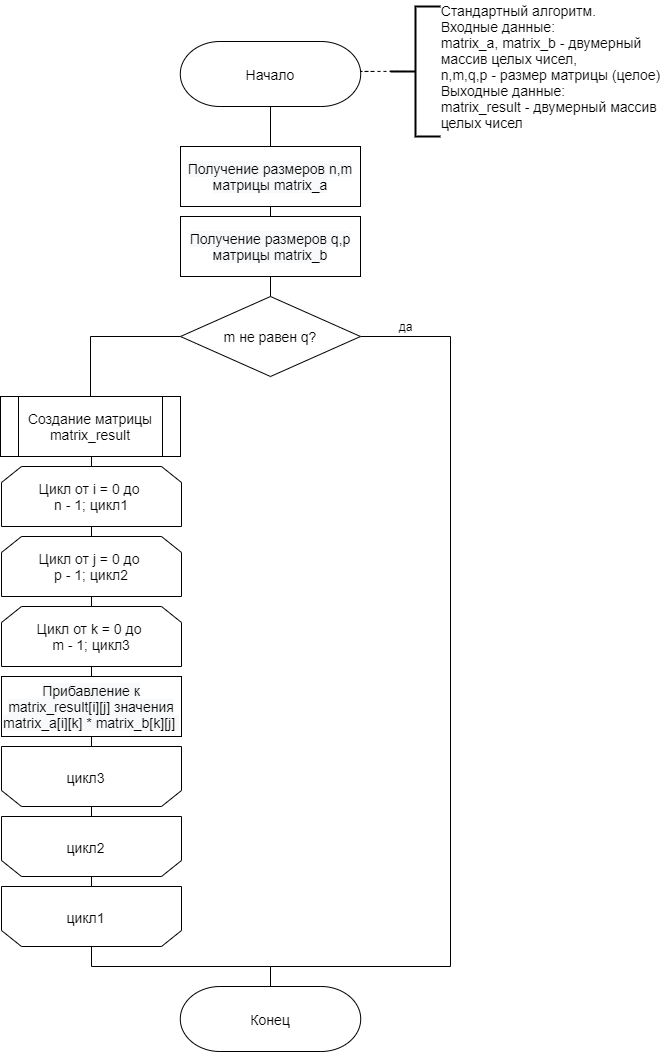
\includegraphics[scale=0.6]{../../../../../../../msys64/home/Лев/bmstu_sem_5_aa/lab_02/report/diagrams/classic}
			\caption{Схема алгоритма стандартного умножения матриц.}
			\label{png:1}}
	\end{figure}
	\newpage
 
	\item рис. \ref{png:2}, \ref{png:3}, \ref{png:4} - схема алгоритма умножения матриц по Винограду;
	\begin{figure}[H]
		\centering{
			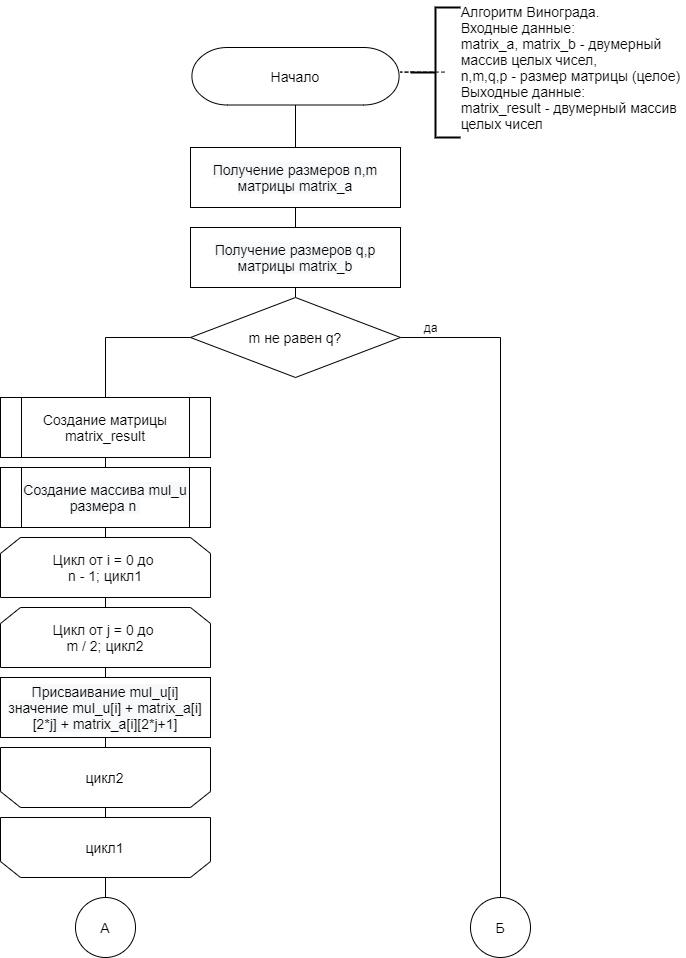
\includegraphics[width=14.6cm]{../../../../../../../msys64/home/Лев/bmstu_sem_5_aa/lab_02/report/diagrams/vinograd_1}
			\caption{Схема алгоритма умножения матриц по Винограду.}
			\label{png:2}}
	\end{figure}

	\begin{figure}[H]
		\centering{
			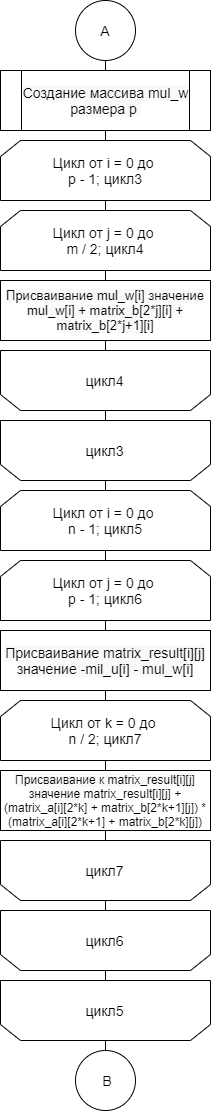
\includegraphics[scale=0.6]{../../../../../../../msys64/home/Лев/bmstu_sem_5_aa/lab_02/report/diagrams/vinograd_2}
			\caption{Схема алгоритма умножения матриц по Винограду.}
			\label{png:3}
		}
	\end{figure}

	\begin{figure}[H]
		\centering{
			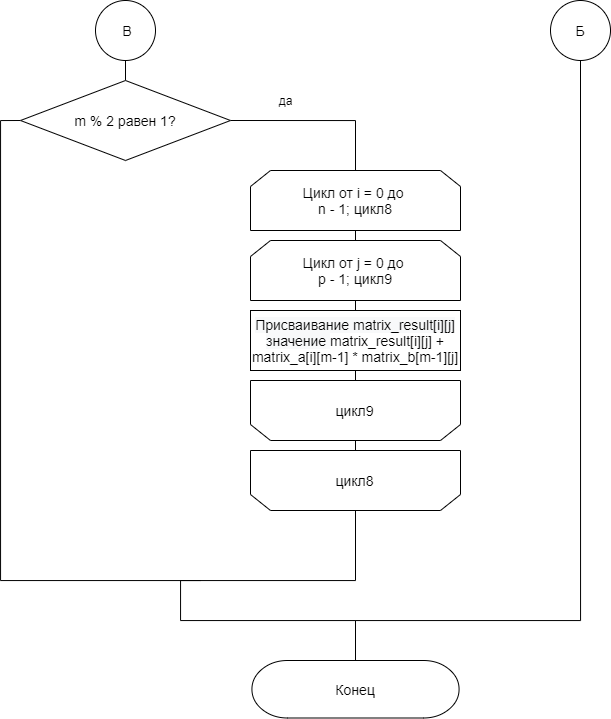
\includegraphics[width=14.6cm]{../../../../../../../msys64/home/Лев/bmstu_sem_5_aa/lab_02/report/diagrams/vinograd_3}
			\caption{Схема алгоритма умножения матриц по Винограду.}
			\label{png:4}
		}
	\end{figure}

	\newpage
	\item рис. \ref{png:5}, \ref{png:6}, \ref{png:7}, \ref{png:8} - схема алгоритма оптимизации алгоритма Винограда.
	\begin{figure}[H]
		\centering{
			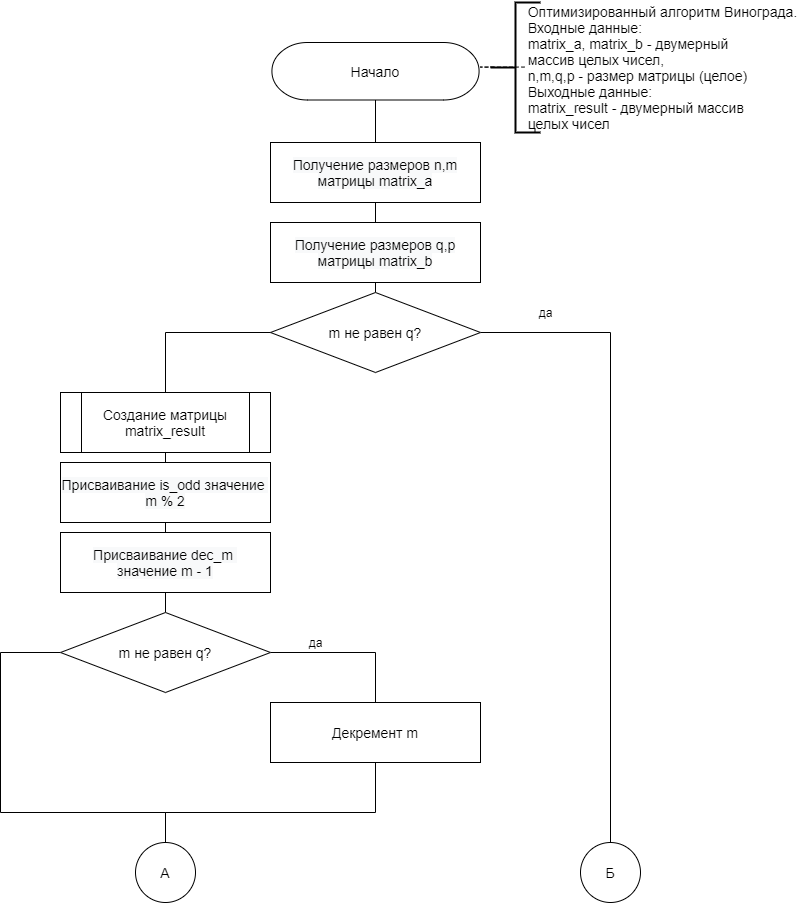
\includegraphics[scale=0.6]{../../../../../../../msys64/home/Лев/bmstu_sem_5_aa/lab_02/report/diagrams/optimized_vinograd_1}
			\caption{Схема алгоритма оптимизации алгоритма Винограда.}
			\label{png:5}
		}
	\end{figure}

	\begin{figure}[H]
		\centering{
			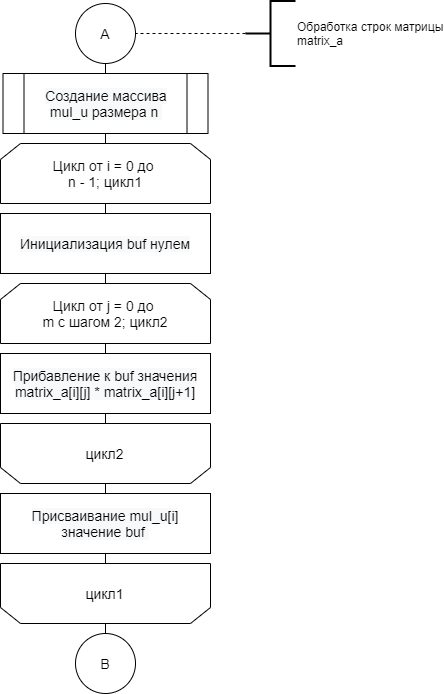
\includegraphics[scale=0.7]{../../../../../../../msys64/home/Лев/bmstu_sem_5_aa/lab_02/report/diagrams/optimized_vinograd_2}
			\caption{Схема алгоритма оптимизации алгоритма Винограда.}
			\label{png:6}
		}
	\end{figure}

	\begin{figure}[H]
		\centering{
			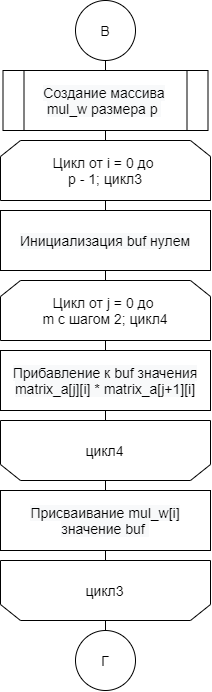
\includegraphics[scale=0.7]{../../../../../../../msys64/home/Лев/bmstu_sem_5_aa/lab_02/report/diagrams/optimized_vinograd_3}
			\caption{Схема алгоритма оптимизации алгоритма Винограда.}
			\label{png:7}
		}
	\end{figure}

	\begin{figure}[H]
		\centering{
			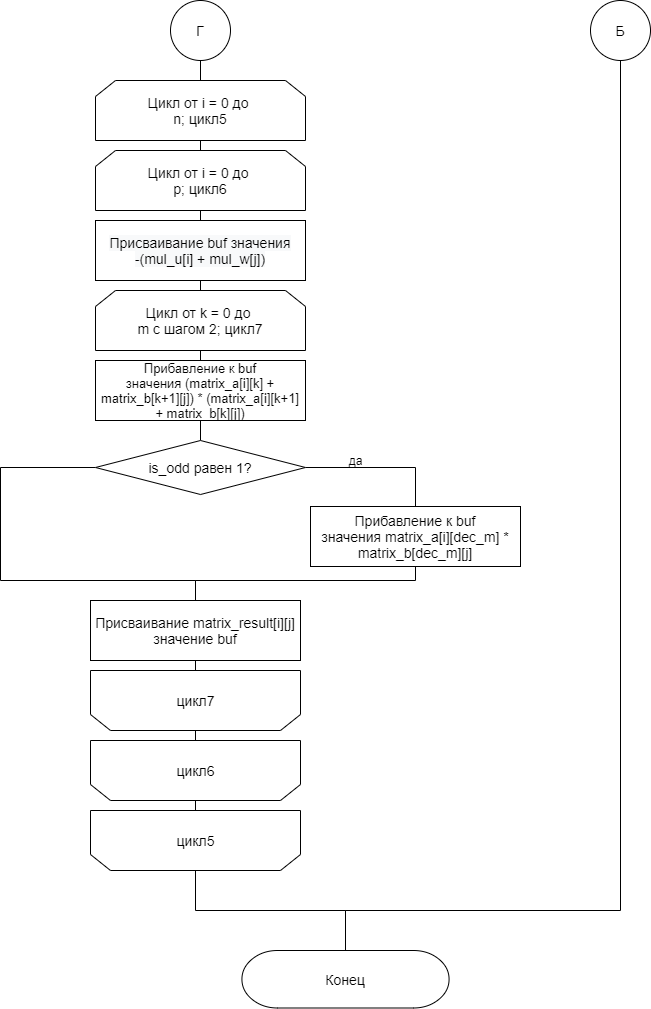
\includegraphics[scale=0.7]{../../../../../../../msys64/home/Лев/bmstu_sem_5_aa/lab_02/report/diagrams/optimized_vinograd_4}
			\caption{Схема алгоритма оптимизации алгоритма Винограда.}
			\label{png:8}
		}
	\end{figure}
\end{itemize}

\section{Вывод}
На основе теоретических данных, полученных в аналитическом разделе, были построены схемы необходимых алгоритмов. Эти алгоритмы были проанализированы с точки зрения трудоемкость выполнения. Алгоритм умножения матриц по Винограду работает медленнее стандартного алгоритма на MNK. Зато оптимизированный вариант алгоритма  Винограда дает выигрыш по сравнению с ним на 6MNK.